% Chapter 7

\chapter{Error Analysis} % Main chapter title
There are various sources of systematic error that could contribute to uncertainty in this measurement. These include certainty in how the event plane was determined (sect. \ref{secteperr}), how well the event centrality can be determined (sect. \ref{sectcenterr}), various uncertainties pertaining to the identification of the particles (sect. \ref{sectpiderr}), and the effects of detector acceptance (sect. \ref{sectaccepterr}). In this chapter I will quantify the uncertainty for each of these contributions and then use these values to find the possible variance in the flow measurement due to these uncertainties. It will be shown that event plane resolution and PID systematics due to Gaussian fitting dominate and other errors are negligible.

Any uncertainty that would affect the value of this flow measurement would do so in one of two ways: either by shifting individual $v_2$ data points (changing inherent shape of the data set) or by changing the overall scaling of the whole measurement in a net direction (simple scaling of entire data set). Errors that would simply shift all values of $v_2$ are the event plane resolution and centrality determination errors. Errors that would shift individual points consist of the various PID uncertainties and detector acceptance effects. The way the uncertainties in this category would shift individual data points is by changing the shape of the particle yield distribution in $d\phi$. Recall that there are two terms that parametrize the shape of the yield in $d\phi$:

\begin{equation}
yield(d\phi) = v_0 [1 + v_2 \cos 2d\phi]
\end{equation}

In this equation, $v_0$ corresponds to an overall shift in the function, that is to say it describes the up-and-down displacement of the whole curve and doesn't affect the general shape of it. The remaining parameter, $v_2$, describes the shape of the yield distribution in $d\phi$. Changes to the shape of this distribution happen when yield values are perturbed up or down in individual bins of $d\phi$ which results in a change in the associated $v_2$. In order to study the strength of $v_2$-affecting uncertainties I will apply the variances discussed in this chapter to individual points in the yield vs $d\phi$ distribution and re-fit with a cosine in order to see the effect varying individual points has on the flow coefficient. 

\section{Event Plane Resolution Correction}
\label{secteperr}
\begin{table}[htbp!]
\centering
\caption[Event Plane Resolution Corrections for MPC, 0-5\% centrality]{Event Plane Resolution Corrections for MPC, 0-5\% centrality, calculated using the Three Sub Event method (see sect. \ref{sect:epres})}
\label{EPrestable}
\begin{tabular}{|l|l|}
\hline
\textbf{Detectors Used}     & \textbf{$\Psi_{RES.3SE}$}       \\ \hline
\textit{MPC, SMD, RXNIN}    & \textit{0.200718 $\pm$ 0.0001312} \\ \hline
\textit{MPC, SMD, RXNOUT}   & \textit{0.261658 $\pm$ 0.0001312} \\ \hline
\textit{MPC, SMD, RXNCMB}   & \textit{0.241446 $\pm$ 0.0001311} \\ \hline
\textbf{$\langle\Psi_{RES.MPC}\rangle$}            & \textbf{0.234607}               \\ \hline
\textbf{$\sigma_{RES.MPC}$} & \textbf{0.03104}                \\ \hline
\end{tabular}
\end{table}
As mentioned in section \ref{sect:epres}, the limitations of the detectors to precisely resolve the event plane result in a weaker anisotropic flow measurement. We therefore define a resolution correction to the overall $v_2$ measurement such that:
\begin{equation}
v_n = \frac{v_n^{A}}{Res(\Psi_n^A)}
\end{equation}
where Res($\Psi_n^A$) is the resolution correction for the n-th order event plane determined using detector A. Because of this definition, detectors that are able to resolve the event plane more precisely require less of a correction, so larger values of resolution correction would come from detectors that are better suited to measure the event plane. These resolution limitations are exacerbated by the asymmetric nature of the d+Au system. From the way ions are fed into RHIC and the orientation of PHENIX in the RHIC ring, the north arm is the ``deuteron-going'' side and the south side is the ``gold-going'' side, i.e. deuteron remnants and forward produced particles hit the north arm and spectators and particles produced from the gold beam hit the south arm. The significant increase in the number of nucleons in a gold nucleus result in higher track multiplicity in the south arm which, in turn, makes the determination the event plane using south arm detectors significantly easier for the d+Au system. This can be seen by comparing the event flattening plots for the north and south detectors in fig \ref{fig:evtpln}. This combination of higher track multiplicity in the south arm and a smooth flattened event plane distribution in the MPC makes it a good choice for event plane determination. Furthermore, because each of the sub event terms in the three sub event method for determining the resolution correction is calculated using the average values for the differences of event plane measurements for two detectors, these average values can be calculated for all combinations of detectors which can, in turn, be used to combinatorially determine the resolution correction for every detector. In doing so, it was seen that the MPC has the best resolution of all the detectors possible. Additional independent measurements of the event plane are used to correct further resolution limitations in the MPC (using the Three Subevent Method, eqn. \ref{eqn3se}). The resolution correction measurements displayed in table \ref{EPrestable} were determined using 5 detectors: the SMD, MPC, inner RXNP, outer RXNP, and the combined RXNP. Since any 3 detectors can be used to determine an event plane resolution correction, this correction can be calculated for the MPC using various detectors as subevent comparisons. This was done using combinations of detectors as listed in the table and the mean was calculated of all combinations. The corresponding variance of this set of measurements can be attributed to systematics inherent in each detector subsystem. Doing so gives a 13\% systematic variance on the MPC resolution correction.

\section{Centrality Resolution}
\label{sectcenterr}
Flow is at its strongest in most central collisions and uncertainty in the determination of centrality could affect the flow measurement. Collaborators have addressed the centrality categorization in Run 8 d+Au\citep{phenixcentrality} by correlating the charge sum in the BBC to the number of binary collisions ($\langle N_{coll} \rangle$). They found a systematic uncertainty of 7\% on the determination of $\langle N_{coll} \rangle$ for this data set for centralities from 0-20\% when compared to Glauber model Monte Carlo simulations. Furthermore, centrality systematics do little to change the shape of the yield vs $d\phi$ distribution and only increase the statistics. As a check, I performed the flow measurement on a centrality range from 0-4\% and 0-6\% to see if the value was changed appreciably or not. In figure \ref{fig:centsys} I have plotted the fractional deviation:
\begin{equation}
\sigma_{sys}^{centrality} = \left| \frac{v_{2}^{0-5\%}-v_{2}^{0-4\%(6\%)}}{v_{2}^{0-5\%}} \right|,
\end{equation}
as a measure of the effect of varying size of the centrality bin on the flow measurement. This deviation was maximally 5\% and appeared to have no correlation to the $p_T$ of the tracks.

\begin{figure}[htbp]
  \centering
    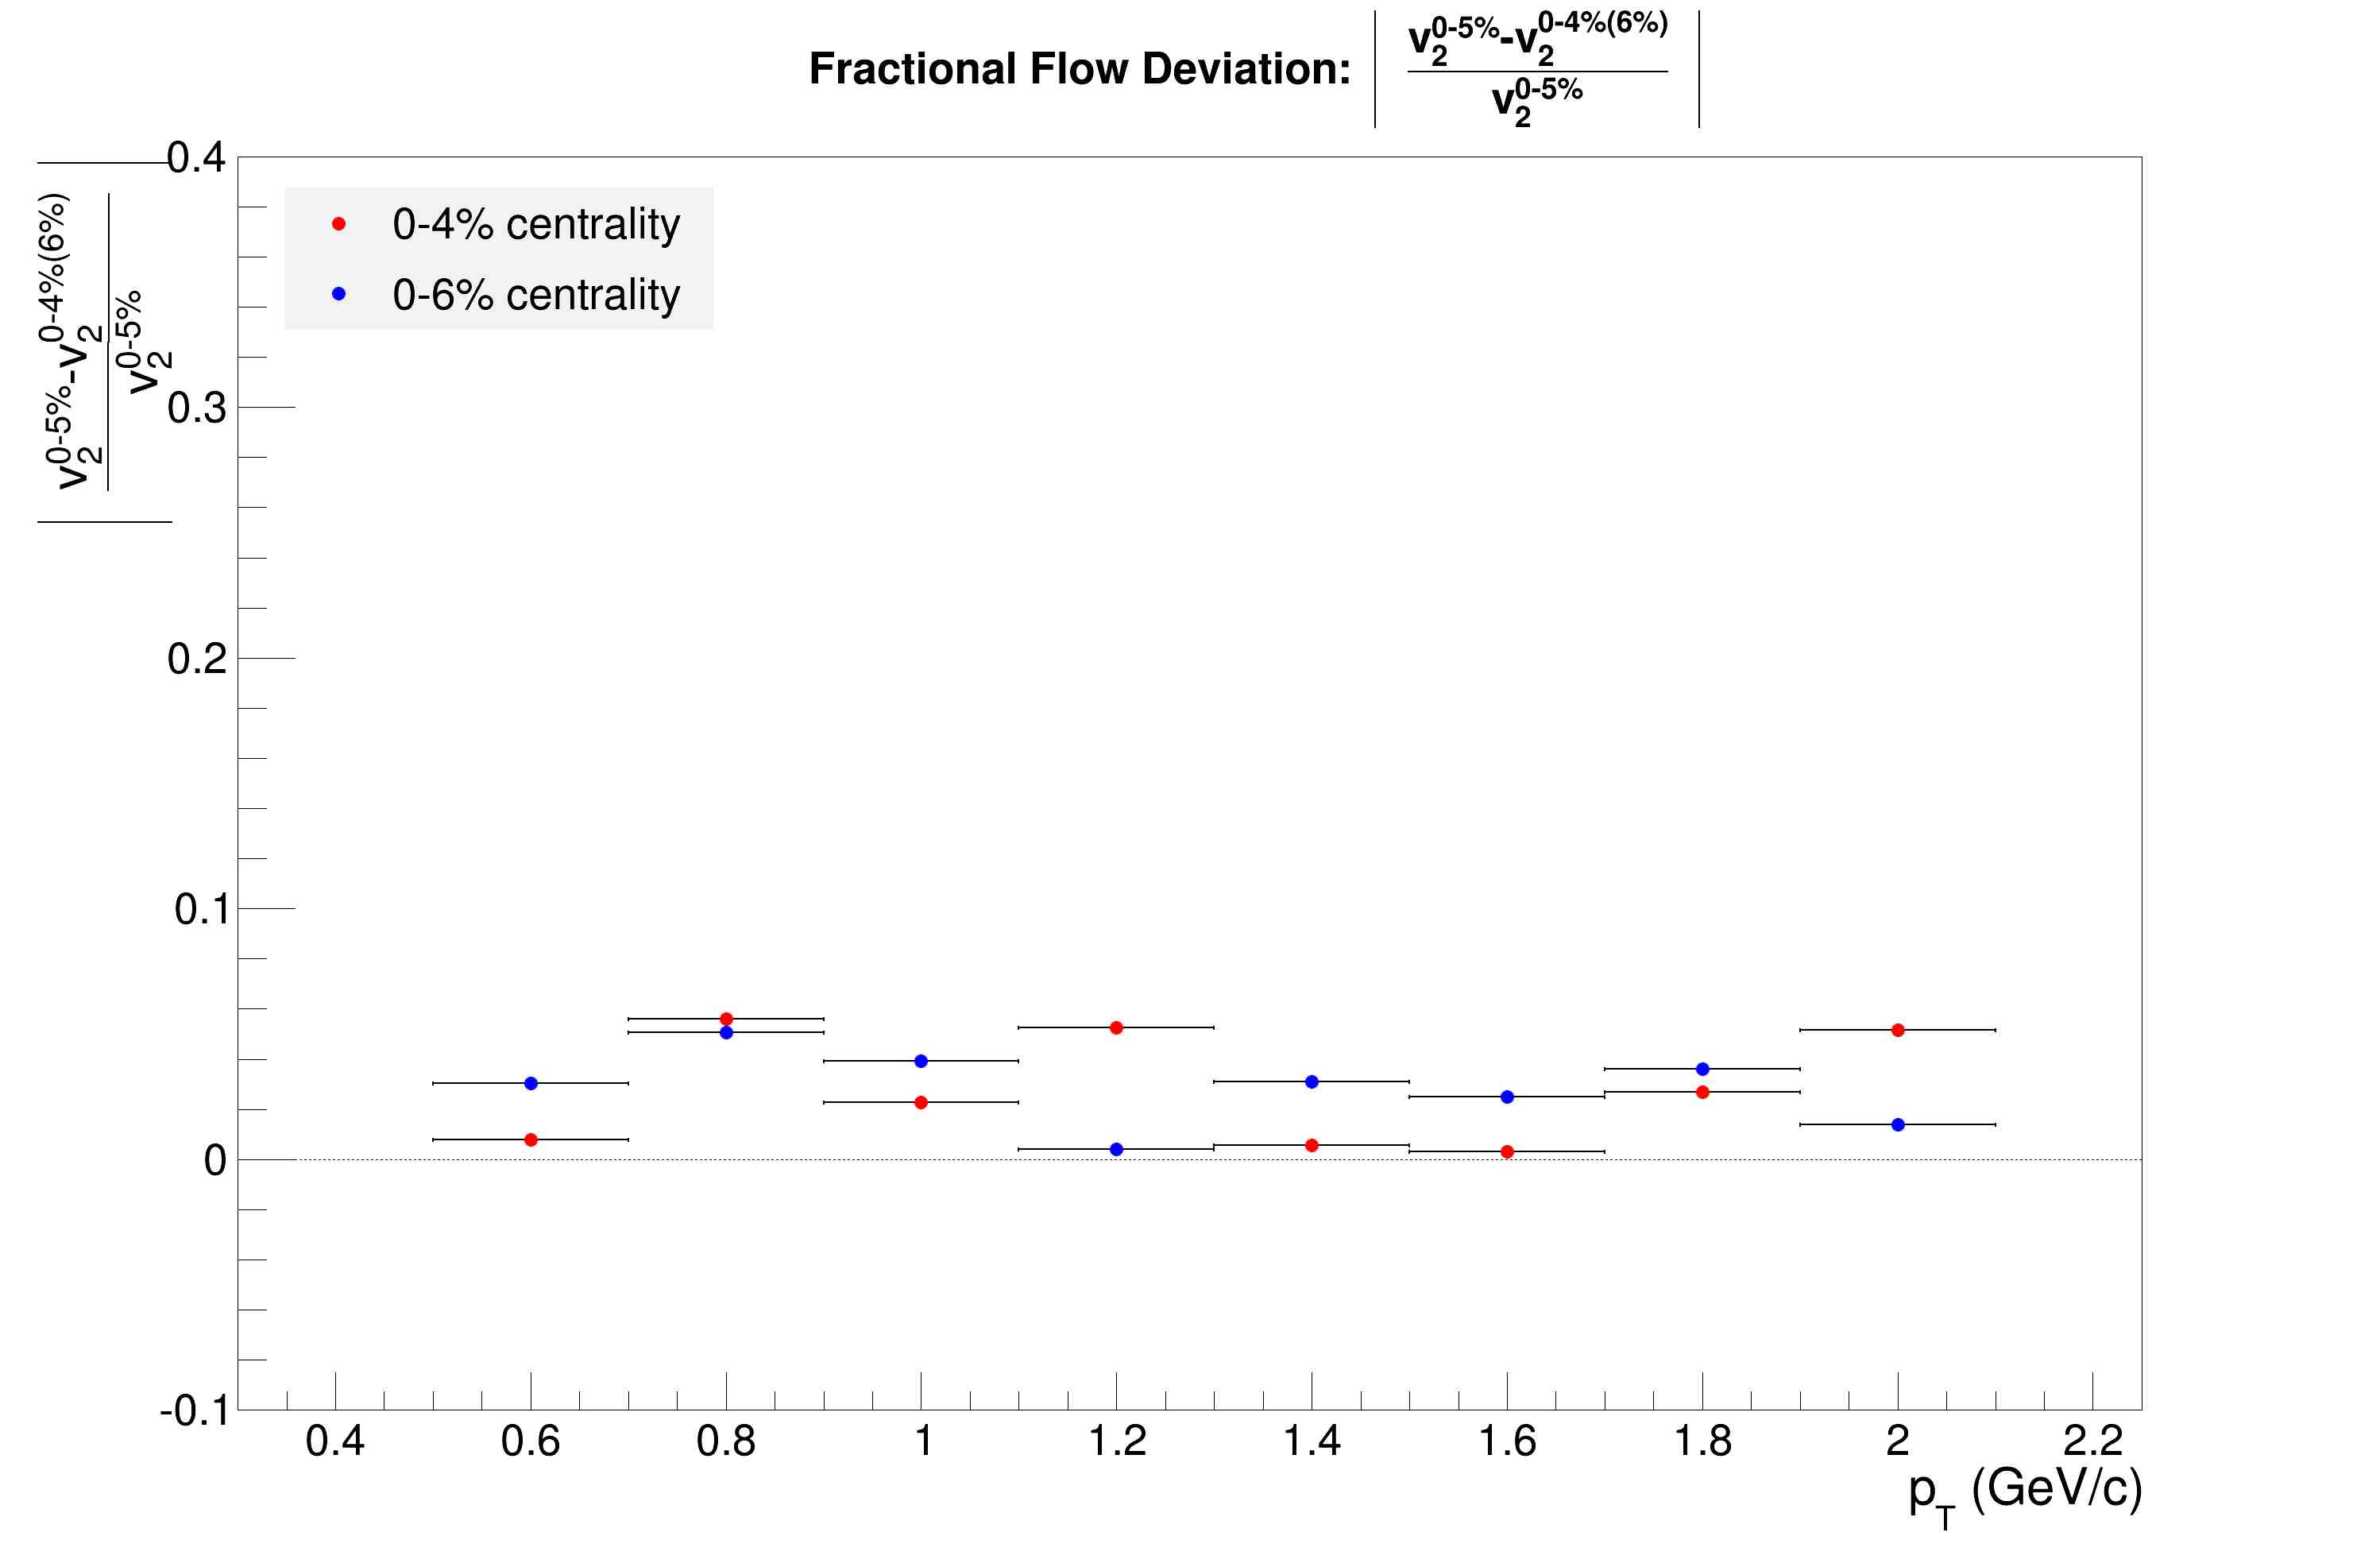
\includegraphics[width=0.8\textwidth]{evtQA/CentSysErrs.jpg}
    \rule{35em}{0.5pt}
  \caption[Centrality uncertainty contribution to Systematic Error]{Centrality uncertainty contribution to Systematic Error}
  \label{fig:centsys}
\end{figure}

\section{Particle Identification Methods}
\label{sectpiderr}
There are three sources of error that can come from the identification of these particle species. Since the separation of signals is dependent on the time of flight and the momentum, uncertainty in either of these propagates to the error in identification. Furthermore, imperfections in the Gaussian fits can systematically miscount particles contributing to further uncertainty in flow coefficients.

\subsection{Momentum Uncertainty}
Track momentum is determined by track curvature in the DC/PC1 as described in section \ref{trkrecosect}. Track curvature and certainty of this calculation is correlated to the ability to match hits in the DC and PC which is quantified by the \textit{track quality} designation. As mentioned, only tracks which have at least 3 hits in the DC and PC1 are accepted for analysis. Additionally, TOF and PC3 tracking adds additional confidence to the tracing of individual hits to reconstructed tracks. Track projections that pass the quality cut in the PC1 are projected onto the TOF and PC3 and only hits that fall within $3\sigma$ of the projected hit are accepted for analysis. Furthermore, momentum reconstruction resolution has been studied with single particle simulations\citep{Mitchell:2002wu}. This resolution was shown to be linear in $p_T$ with the highest $p_T$ bin used in this analysis (5 GeV/c) having a resolution of 2\%.
 
\subsection{TOF Timing}
Since the TOF boasts a very high timing resolution and since the preamplifier gains, cable lengths, and various other systematics can affect the timing measurement from strip to strip, it is important to calibrate the response across all the strips in the TOF. Conventionally, the tracks are shifted to some expected value. Since pions are by far the most plentiful particles created in heavy ion collisions, we pick them to be our normalization. Specifically, the track time distribution is plotted for each strip individually. We know the start of the event time as given by the BBC and we know the expected time of flight for a pion ($t_{\pi}$) of mass $m_{\pi}$ with a measured momentum, $p$:

\begin{equation}
t_{\pi} = \sqrt{\frac{m_{\pi}}{p^2} + \frac{1}{c^2}}.
\end{equation}

Each strip is then fit with a normal distribution and the distance from the mean to $t=0$ is the timing offset ($\Delta t$) for the strip. This offset is then applied to each track's measured time:

\begin{equation}
\Delta t = t_{TOF measured} - t_{collision/BBC} - t_{\pi} 
\end{equation}
 
\begin{figure}[htbp]
  \centering
    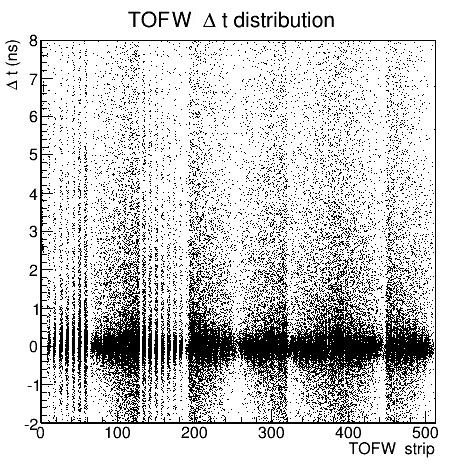
\includegraphics[width=0.7\textwidth]{evtQA/ttofwdist.JPG}
    \rule{35em}{0.5pt}
  \caption[Timing QA in the TOF.W]{Timing QA in the TOF.W, $\Delta$t vs TOF.W strip id}
  \label{fig:tofwdist}
\end{figure}

\begin{figure}[htbp]
  \centering
    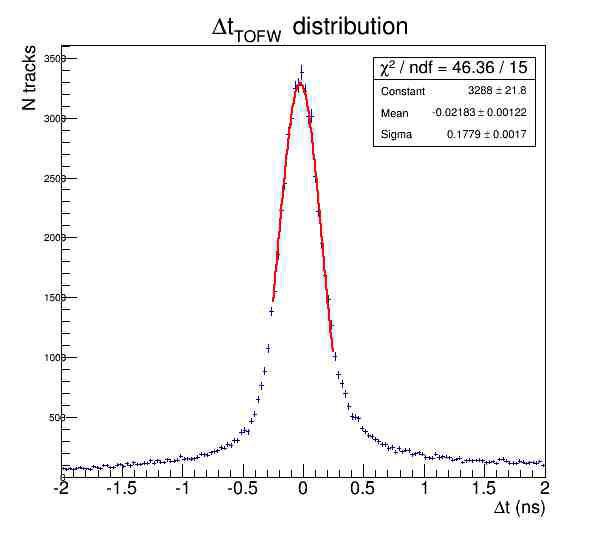
\includegraphics[width=0.7\textwidth]{evtQA/deltattofwdist.jpg}
    \rule{35em}{0.5pt}
  \caption[Systematic Offset in TOF.W]{Systematic Timing Offset in the TOF.W}
  \label{fig:tofwsyst}
\end{figure}

Given the TOFW's known resolution of $\sim 80 ps$, if we propagate this error through eqn. \ref{eqn:m2tof} with the known distance from the vertex of the TOF.W and a maximal $p_T$ value for this analysis of 5 GeV/c, the maximum variance in $m$ due to resolution is $\pm 2$ eV/c$^2$) which, when compared to the smallest mass measured ($m_{\pi}\approx$139 MeV/c$^2$), is negligible. Furthermore, the systematic offset of the detector after calibration is 21 ps, well below the TOFW's resolution limitation (fig. \ref{fig:tofwsyst}).

\subsection{Uncertainties from Gaussian Models}
\subsubsection{Single and Mixed Gaussians, no ACC, $p_T\leq2.1$ GeV/c}
Species purity is integrated out to $2\sigma$ which accounts for 95.45\% of particles about the mean of their distribution. Therefore, systematics due to mixing in the tails of the particle distributions is at most 4.55\%. Gaussian distributions do not perfectly match the particle distributions, often there is a tradeoff between fitting the shape of the peak or the shape of the tails. Given the $2-\sigma$ integration of the Gaussians, fitting the shape of the peaks took priority as the tails would contribute very minimally. This systematic uncertainty in the tails always \textit{under} counts the number of particles in a distribution, however it can be seen from inspection (see App. \ref{app:data}) that and over and under counting done by the models is uniform across each bin in $d\phi$ for within the same bin of $p_T$. Any systematic over/under counting such as this only serves to shift the y-position of the flow curve a net value up or down without changing the value of the harmonic. This appears to remain true for $p_T \leq 2.1$ GeV/c. There are a few instances where fitting algorithms appear to have not matched the shape of the peaks perfectly but the functions fit nicely through the waist of the distribution. Each of these bins were inspected and allowed to vary by hand to fit various misshapen regions of the distributions. The maximal variance in the yield from the fit functions was 2\% for the pions and kaons and $<$1\% for the protons in this range of $p_T$.

\subsubsection{ACC Meson Separation and Gaussian Tail Cross Contamination, $2.1\leq p_T \leq 2.9$}
For $p_T \geq 2.1 GeV/c$, the ACC is used to separate pions from kaons and protons. Over/under counting in the tails is still the most likely place for systematic errors to accrue and this effect is strongest in the kaons since the ACC threshold still allows some pion contamination. Because of this, fitting the peaks and the right side waist and tail of the kaon distributions for ACC vetoed tracks took priority. In the lower bound of this $p_T$ range, kaons maintain good separation from protons, however as the $p_T$ increases there is some species contamination in the tails. This is accounted for in two ways. Firstly, as with the low $p_T$ $\pi / k$, mixing happens in the extremes of the tails and particle counting stops at $2-\sigma$. Secondly. A two peak, Mixed Gaussian model is used to fit the kaon and proton peaks which allows for the additive overlap in the tails to be visualized and accounted for. This accounts for a 5\% maximum systematic error for the kaons and 2\% max for the protons. Since the ACC operates on Cherenkov radiation, the ``ACC fire'' condition is far more selective since it requires particles to be traveling fast enough to radiate. This leads to a very pure pion signal with negligible contamination, attributing $<1\%$ systematic uncertainty.

\subsubsection{Fixed Width/Mean Gaussians and Background Effects}
For $p_T \geq 3$ GeV/c, low statistics cause the means and widths of particle distributions to vary across bins in $d\phi$. Because of this, all $d\phi$ bins are summed for a given $p_T$ bin and are fit as a whole in order to fix a constant mean and width for each particle species. In doing so, only the heights of the Gaussians are allowed to vary. In practice, this method tends to undercount particles. When the means of particle distributions deviate from the model-fixed values of the Gaussian models it causes only the regions that fall under the Gaussians to be counted, largely missing regions of the distribution that are not encompassed by the curve. This accounts for a 7\% under-counting in these bins.

Additionally, background tracks for the very last $p_T$ bin are strong enough to contribute to error. The TOFW along with the PC3 allows for very strong background rejection thanks to the two detectors' high precision tracking and distance from the event vertex. Only tracks with five matching points are accepted for analysis, that is: 2 hits in the DC, 1 matched hit in the PC1 within $2-\sigma$, 1 matched hit in the TOFW within $3-\sigma$, and 1 matched hit in the PC3 to $3-\sigma$. This leads to a negligible background for high statistics analyses. For $4\leq p_T \leq4.5$, the numbers of detected particles are low enough that the background may contribute 1 out of every 10 tracks counted for each particle species. This leads to a 10\% systematic error for this last bin from background.

\section{Detector Acceptance}
\label{sectaccepterr}
Detectors occupy a limited and constant range in space. The ability of a detector to cover a range in space is called its \textit{acceptance}. Additionally, detectors are imperfect, there are dead channels, hot channels, edge effects, and other phenomena that can ruin the efficiency of a detector and add holes to its acceptance. Because of this, acceptance limitations of detectors can affect measurements in various analyses, however, for reasons I will discuss, a flow analysis is at best negligibly affected by detector acceptance effects. Analyses where acceptance effects are strongest are those where the coordinate system is ``static''. By this I mean that the production of analyzed tracks are studied in the lab frame coordinate system and any repeatedly missed tracks in a hole in acceptance are missed indefinitely and completely. Since event characteristics are random, by the necessity of event plane determination there is a statistical ``smearing'' that happens from the Q-vector normalization and the event plane flattening. Any holes in azimuthal coverage due to detector limitations in the lab coordinate system are smeared over by this normalization and flattening since we are performing the analysis in the event plane coordinate system which is statistically distributed and normalized. Furthermore, collaborators have studied the systematics of acceptance on $v_2$ measurements\citep{azianisystematics} by comparing $v_2$ measurements made with charged hadrons detected in TOF.E and TOF.W ($45^{\circ}$ per arm) with charged hadrons detected in full central arm acceptance ($90^{\circ}$ per arm). They found that a two-fold increase in azimuthal acceptance resulted in less than 2\% difference in flow measurements. 

\section{Summary}
The particle yield is binned in six bins of $d\phi$ which therefore means that there are six points that can be perturbed systematically. In order to study the propagation of the yield uncertainty to the measured flow coefficient I take the known values of yield in $d\phi$ and perturb them up or down by the percentages quantified in this chapter. The changed yield vs $d\phi$ distribution is re-fit and a new flow coefficient is calculated. This new $v_2$ is compared to the original one in order to determine systematic errors on the final measurement which are caused by sources within the process of measuring it. Since the identified track flow follows the behavior of the individual particle flows, I will use it for this study and, for completeness, perturbations both up and down will be studied. 


\begin{figure}[p]
\captionsetup{width=1.2\linewidth}
    \caption[Effects of Systematic Shifts in Yield on $v_2$.]{Effects of Systematic Shifts in Yield on $v_2$. 1\%, 2\%, 4\%, 5\%, 7\%, and 10\% perturbations are applied to each yield for a particular bin of $d\phi$ and the corresponding $v_2$ is calculated. Closed circles are downward perturbations, open circles, upward perturbations.}
    \rule{35em}{0.5pt}
    \centerline{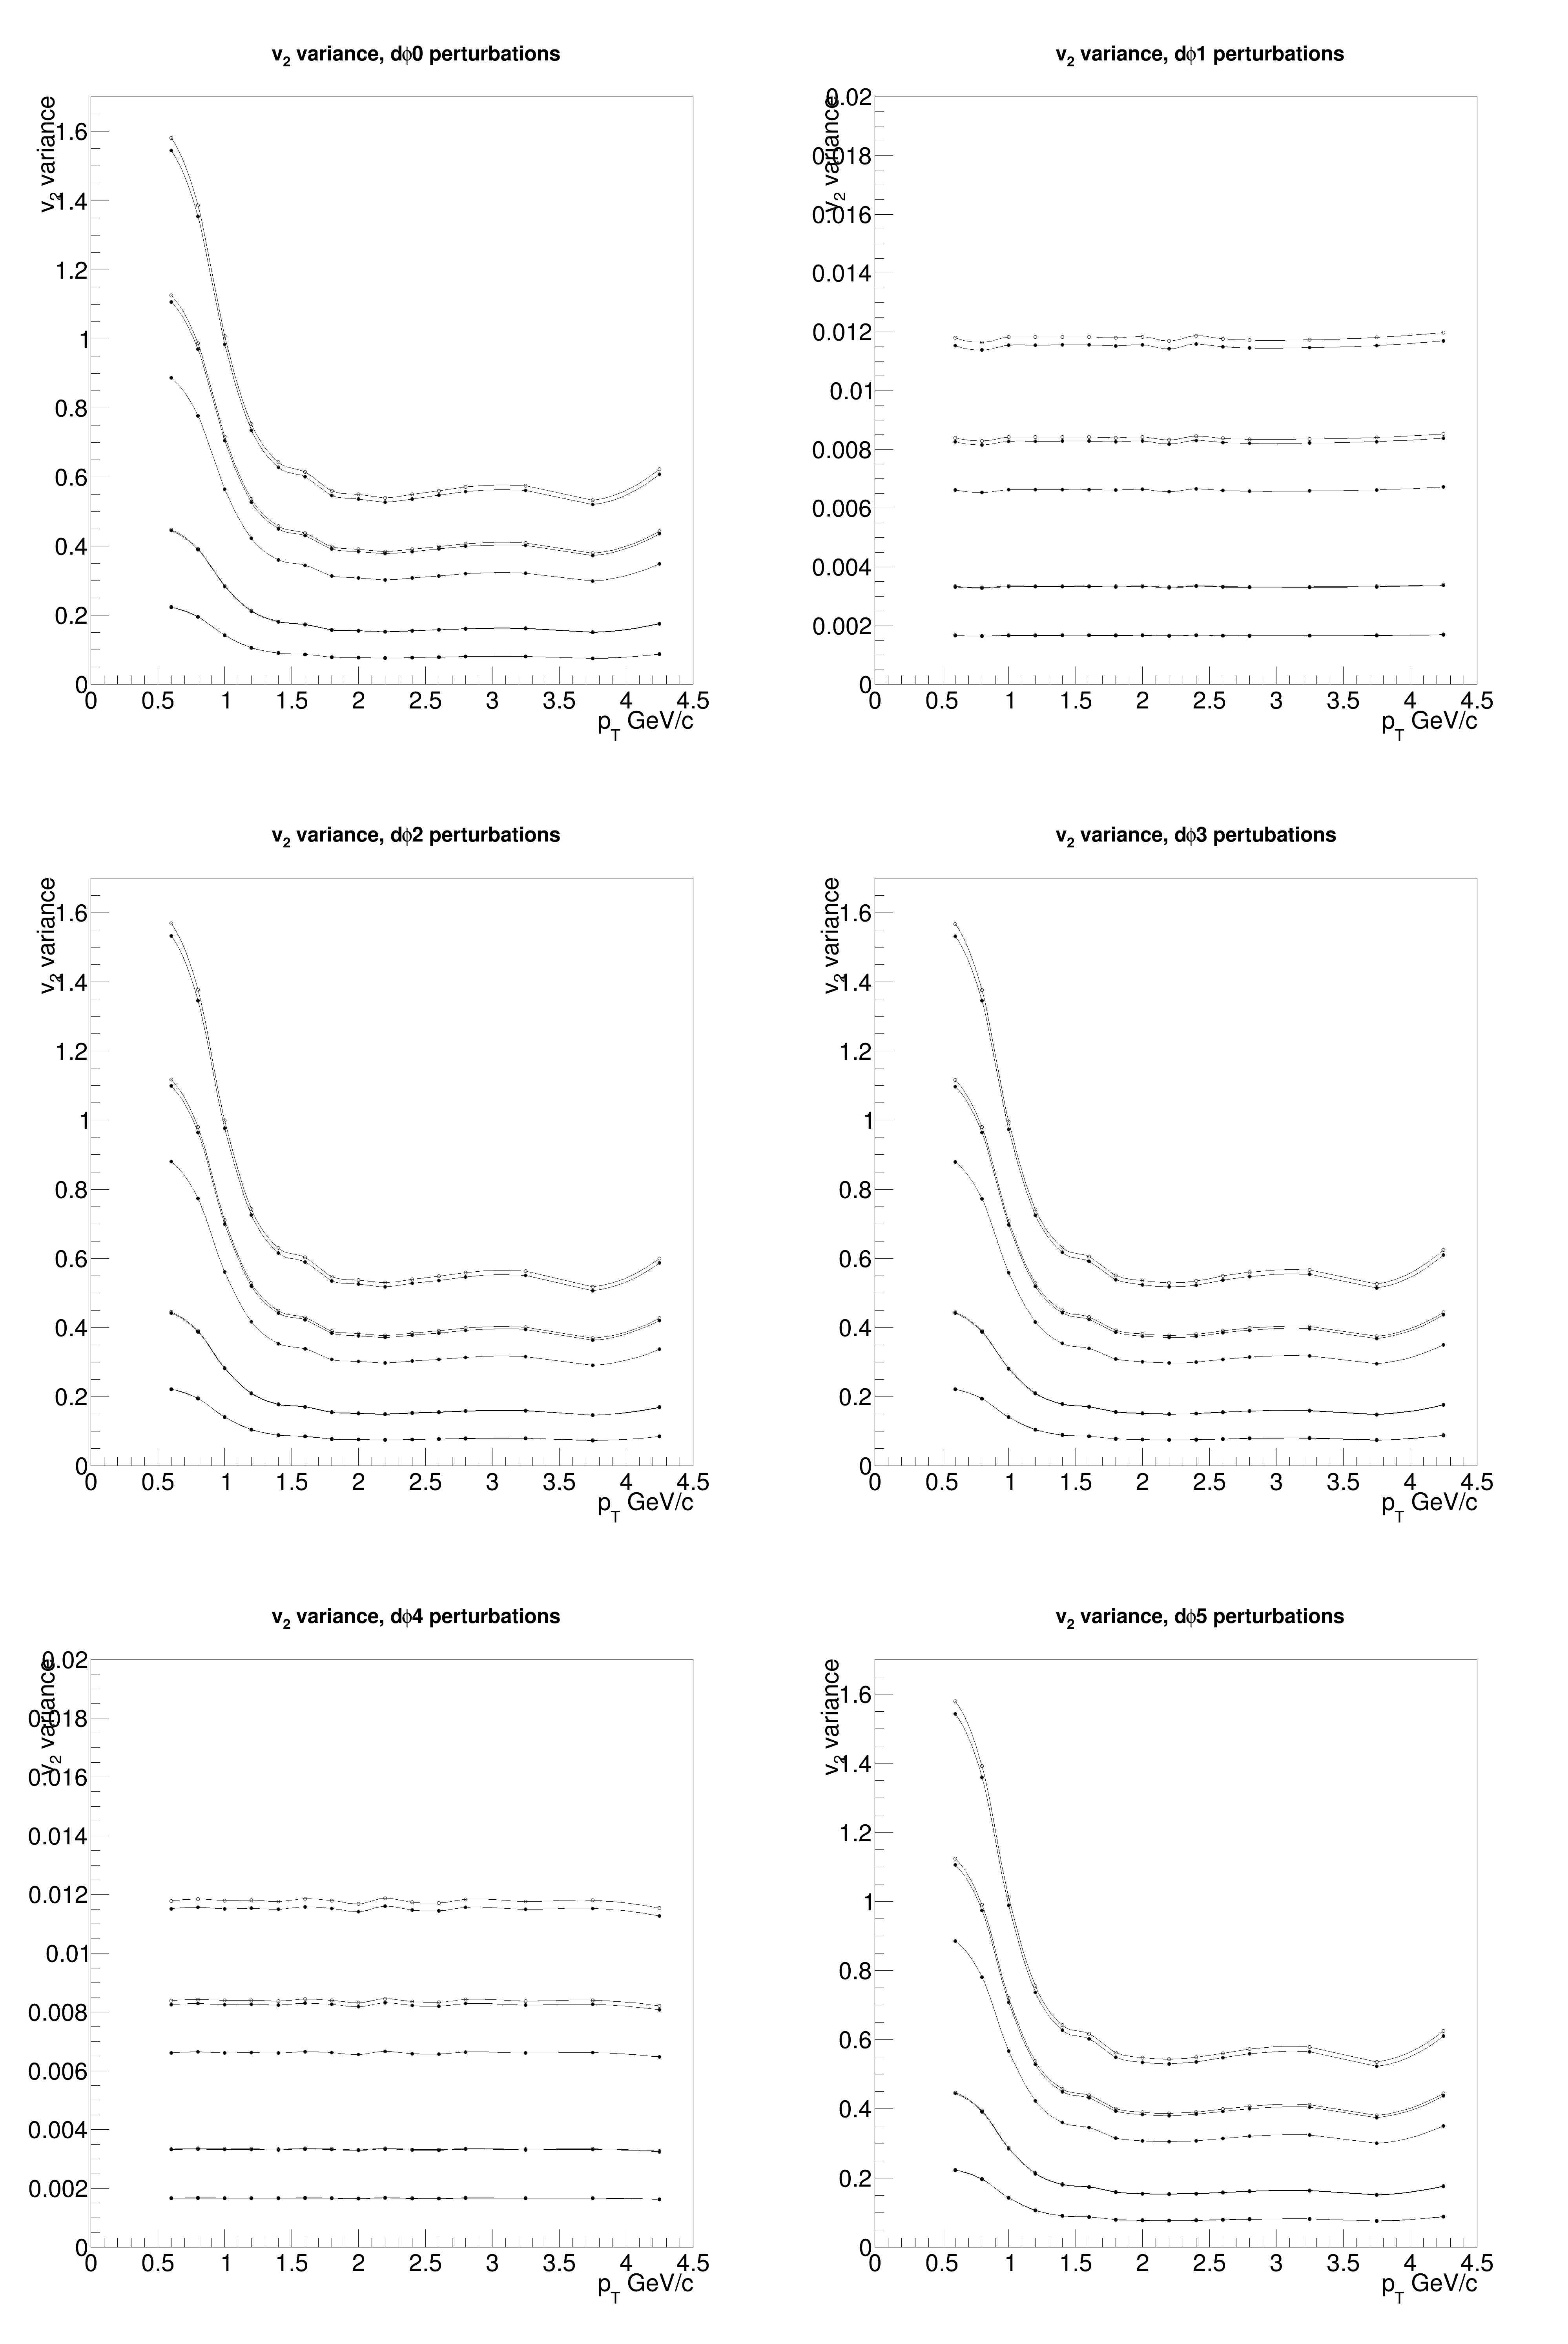
\includegraphics[width=1\textwidth]{evtQA/plusminusstudy.jpg}}
    \label{fig:wiggleupdown}
\end{figure}

In practice, of these six points, four contribute strongly to the overall shape of the yield distribution, these are: the two end points and the two center points. This is shown by the significantly smaller systematic error in bins 1 and 4 in fig \ref{fig:wiggleupdown}. Additionally, the direction of perturbation makes a negligible difference; up and down perturbations line up very well on the plots. Yield systematics have the strongest effect on the lower $p_T$ bins. This is because their significantly higher statistics correspond to a larger loss or gain of counted particles with which to skew the flow coefficient.

The resulting systematic errors are summarized in table \ref{tab:syserr}.

\begin{table}[hp]
\centering
\caption{Table of Systematic Errors in each bin of $p_T$}
\label{tab:syserr}
\resizebox{\textwidth}{!}{
\begin{tabular}{lllllllll}
                                                                       & \multicolumn{8}{c}{\textbf{Transverse Momentum Bin Range (GeV/c)}}                                                                                                                                                                                                                                                                                                                                                                                                                                                            \\ \hline \hline
\rowcolor[HTML]{C0C0C0} 
\multicolumn{1}{|l||}{\cellcolor[HTML]{C0C0C0}\textbf{Source of Error}} & \multicolumn{1}{l|}{\cellcolor[HTML]{C0C0C0}\textbf{0.5-0.7}} & \multicolumn{1}{|l|}{\cellcolor[HTML]{C0C0C0}\textbf{0.7-0.9}} & \multicolumn{1}{|l|}{\cellcolor[HTML]{C0C0C0}\textbf{0.9-1.1}} & \multicolumn{1}{|l|}{\cellcolor[HTML]{C0C0C0}\textbf{1.1-1.3}} & \multicolumn{1}{|l|}{\cellcolor[HTML]{C0C0C0}\textbf{1.3-1.5}} & \multicolumn{1}{|l|}{\cellcolor[HTML]{C0C0C0}\textbf{1.5-1.7}} & \multicolumn{1}{|l|}{\cellcolor[HTML]{C0C0C0}\textbf{1.7-1.9}} & \multicolumn{1}{|l|}{\cellcolor[HTML]{C0C0C0}\textbf{1.9-2.1}} \\ \hline \hline
\multicolumn{1}{|l||}{\textbf{Event Plane Resolution}}                  & \multicolumn{1}{l|}{23.40\%}                                  & \multicolumn{1}{l|}{23.40\%}                                  & \multicolumn{1}{l|}{23.40\%}                                  & \multicolumn{1}{l|}{23.40\%}                                  & \multicolumn{1}{l|}{23.40\%}                                  & \multicolumn{1}{l|}{23.40\%}                                  & \multicolumn{1}{l|}{23.40\%}                                  & \multicolumn{1}{l|}{23.40\%}                                  \\ \hline
\multicolumn{1}{|l||}{\textbf{Detector Acceptance}}                     & \multicolumn{1}{l|}{\textless2\%}                             & \multicolumn{1}{l|}{\textless2\%}                             & \multicolumn{1}{l|}{\textless2\%}                             & \multicolumn{1}{l|}{\textless2\%}                             & \multicolumn{1}{l|}{\textless2\%}                             & \multicolumn{1}{l|}{\textless2\%}                             & \multicolumn{1}{l|}{\textless2\%}                             & \multicolumn{1}{l|}{\textless2\%}                             \\ \hline
\multicolumn{1}{|l||}{\textbf{Centrality Determination}}                & \multicolumn{1}{l|}{5\%}                                      & \multicolumn{1}{l|}{5\%}                                      & \multicolumn{1}{l|}{5\%}                                      & \multicolumn{1}{l|}{5\%}                                      & \multicolumn{1}{l|}{5\%}                                      & \multicolumn{1}{l|}{5\%}                                      & \multicolumn{1}{l|}{5\%}                                      & \multicolumn{1}{l|}{5\%}                                      \\ \hline
\multicolumn{1}{|l||}{\textbf{PID uncertainty (pion)}}                  & \multicolumn{1}{l|}{22\%}                                     & \multicolumn{1}{l|}{20\%}                                     & \multicolumn{1}{l|}{14\%}                                     & \multicolumn{1}{l|}{11\%}                                     & \multicolumn{1}{l|}{9\%}                                      & \multicolumn{1}{l|}{17\%}                                     & \multicolumn{1}{l|}{16\%}                                     & \multicolumn{1}{l|}{15\%}                                     \\ \hline
\multicolumn{1}{|l||}{\textbf{PID uncertainty (kaon)}}                  & \multicolumn{1}{l|}{22\%}                                     & \multicolumn{1}{l|}{20\%}                                     & \multicolumn{1}{l|}{14\%}                                     & \multicolumn{1}{l|}{11\%}                                     & \multicolumn{1}{l|}{9\%}                                      & \multicolumn{1}{l|}{17\%}                                     & \multicolumn{1}{l|}{16\%}                                     & \multicolumn{1}{l|}{15\%}                                     \\ \hline
\multicolumn{1}{|l||}{\textbf{PID uncertainty (proton)}}                & \multicolumn{1}{l|}{22\%}                                     & \multicolumn{1}{l|}{20\%}                                     & \multicolumn{1}{l|}{14\%}                                     & \multicolumn{1}{l|}{10\%}                                     & \multicolumn{1}{l|}{9\%}                                      & \multicolumn{1}{l|}{8\%}                                      & \multicolumn{1}{l|}{8\%}                                      & \multicolumn{1}{l|}{7\%}                                      \\ \hline
\end{tabular}}

\vspace{1cm}
\resizebox{\textwidth}{!}{
\begin{tabular}{llllllll}
                                                                       & \multicolumn{7}{c}{\textbf{Transverse Momentum Bin Range (GeV/c)}}                                                                                                                                                                                                                                                                                                                                                                                            \\ \hline \hline
\rowcolor[HTML]{C0C0C0} 
\multicolumn{1}{|l||}{\cellcolor[HTML]{C0C0C0}\textbf{Source of Error}} & \multicolumn{1}{l|}{\cellcolor[HTML]{C0C0C0}\textbf{2.1-2.3}} & \multicolumn{1}{l|}{\cellcolor[HTML]{C0C0C0}\textbf{2.3-2.5}} & \multicolumn{1}{l|}{\cellcolor[HTML]{C0C0C0}\textbf{2.5-2.7}} & \multicolumn{1}{l|}{\cellcolor[HTML]{C0C0C0}\textbf{2.7-2.9}} & \multicolumn{1}{l|}{\cellcolor[HTML]{C0C0C0}\textbf{3.0-3.5}} & \multicolumn{1}{l|}{\cellcolor[HTML]{C0C0C0}\textbf{3.5-4.0}} & \multicolumn{1}{l|}{\cellcolor[HTML]{C0C0C0}\textbf{4.0-4.5}} \\ \hline \hline
\multicolumn{1}{|l||}{\textbf{Event Plane Resolution}}                  & \multicolumn{1}{l|}{23.40\%}                                  & \multicolumn{1}{l|}{23.40\%}                                  & \multicolumn{1}{l|}{23.40\%}                                  & \multicolumn{1}{l|}{23.40\%}                                  & \multicolumn{1}{l|}{23.40\%}                                  & \multicolumn{1}{l|}{23.40\%}                                  & \multicolumn{1}{l|}{23.40\%}                                  \\ \hline
\multicolumn{1}{|l||}{\textbf{Detector Acceptance}}                     & \multicolumn{1}{l|}{\textless2\%}                             & \multicolumn{1}{l|}{\textless2\%}                             & \multicolumn{1}{l|}{\textless2\%}                             & \multicolumn{1}{l|}{\textless2\%}                             & \multicolumn{1}{l|}{\textless2\%}                             & \multicolumn{1}{l|}{\textless2\%}                             & \multicolumn{1}{l|}{\textless2\%}                             \\ \hline
\multicolumn{1}{|l||}{\textbf{Centrality Determination}}                & \multicolumn{1}{l|}{5\%}                                      & \multicolumn{1}{l|}{5\%}                                      & \multicolumn{1}{l|}{5\%}                                      & \multicolumn{1}{l|}{5\%}                                      & \multicolumn{1}{l|}{5\%}                                      & \multicolumn{1}{l|}{5\%}                                      & \multicolumn{1}{l|}{5\%}                                      \\ \hline
\multicolumn{1}{|l||}{\textbf{PID uncertainty (pion)}}                  & \multicolumn{1}{l|}{7\%}                                      & \multicolumn{1}{l|}{7\%}                                      & \multicolumn{1}{l|}{8\%}                                      & \multicolumn{1}{l|}{8\%}                                      & \multicolumn{1}{l|}{40\%}                                     & \multicolumn{1}{l|}{40\%}                                     & \multicolumn{1}{l|}{90\%}                                     \\ \hline
\multicolumn{1}{|l||}{\textbf{PID uncertainty (kaon)}}                  & \multicolumn{1}{l|}{35\%}                                     & \multicolumn{1}{l|}{35\%}                                     & \multicolumn{1}{l|}{35\%}                                     & \multicolumn{1}{l|}{35\%}                                     & \multicolumn{1}{l|}{55\%}                                     & \multicolumn{1}{l|}{53\%}                                      & \multicolumn{1}{l|}{90\%}                                     \\ \hline
\multicolumn{1}{|l||}{\textbf{PID uncertainty (proton)}}                & \multicolumn{1}{l|}{15\%}                                     & \multicolumn{1}{l|}{15\%}                                     & \multicolumn{1}{l|}{16\%}                                     & \multicolumn{1}{l|}{16\%}                                     & \multicolumn{1}{l|}{55\%}                                     & \multicolumn{1}{l|}{53\%}                                      & \multicolumn{1}{l|}{90\%}                                     \\ \hline
\end{tabular}}

\end{table}



\pagebreak
\pagebreak
